\begin{frame}
    \frametitle{Introducción}

        \begin{block}{Juegos de conducción}
            \begin{itemize}
                \item Adictivos
                \item Para todo tipo de jugadores
                \item Cortos tiempos de juego
                \item Variados modos de juego
                \item No pasan de moda
            \end{itemize}
        \end{block}

    \begin{columns}
    
        \column{150px}
        %\begin{center}
                %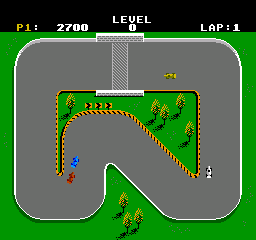
\includegraphics[scale=0.4]{imagenes/super_sprint.png}
        %\end{center}

        \begin{figure}
          \label{logo_latex}
          \begin{center}
            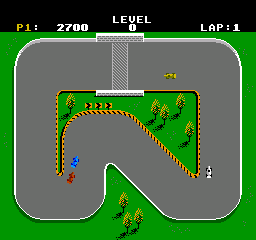
\includegraphics[scale=0.4]{imagenes/super_sprint.png}
          \end{center}
          Super Sprint - Atari (1986)
        \end{figure}
    
        \column{150px}
        \begin{figure}
          \label{logo_latex}
          \begin{center}
            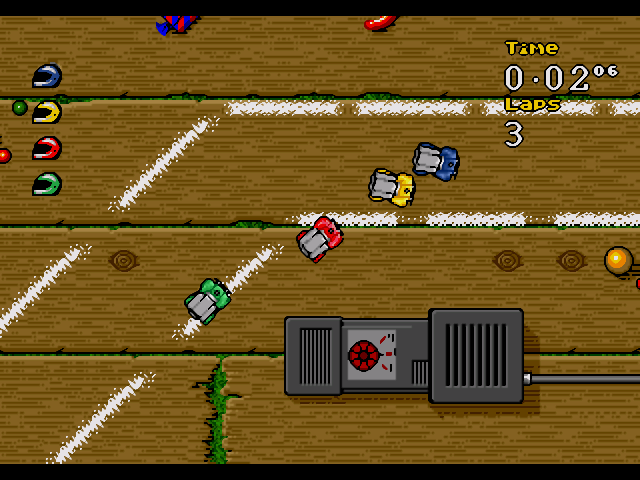
\includegraphics[scale=0.2]{imagenes/micromachines.png}
          \end{center}
          Micromachines - NES (1991)
        \end{figure}

    \end{columns}
    
\end{frame}

\begin{frame}
    \frametitle{Introducción}

    \begin{columns}
    
        \column{150px}
        \begin{block}{Zycars}
            \begin{itemize}
                \item Juego de conducción en 2D con vista cenital
                \item Tres modo de juego
                \item Uso de ítem durante las carreras
            \end{itemize}
        \end{block}

        \column{150px}
        \begin{figure}
          \label{logo_latex}
          \begin{center}
            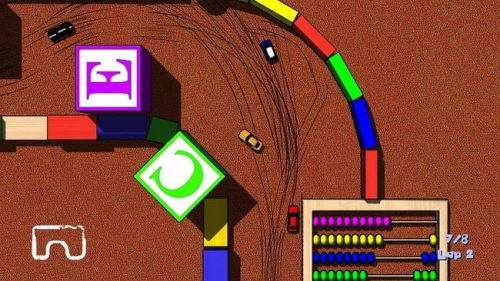
\includegraphics[scale=0.3]{imagenes/toy_cars.jpg}
          \end{center}
          Toy Cars - Xbox 360 (2011)
        \end{figure}
        
    \end{columns}


    \begin{block}{¿Por qué este proyecto?}
        \begin{itemize}
            \item Muy pocos juegos libre con las mismas características
            \item Interés por el mundo de los videojuegos
            \item Cursar la asignatura de Diseño de Videojuegos aumentó el interés por el desarrollo de estos
            \item Contribuir al mundo del software libre
        \end{itemize}
    \end{block}

\end{frame}

\begin{frame}
    \frametitle{Introducción}

    \begin{block}{Objetivos}
        \begin{itemize}
            \item Realizar un juego de coches completamente funcional
            \item Dificultad progresiva (adicción por aprendizaje)
            \item Competidores aceptables, que proponga un desafío
            \item Fácilmente ampliable
        \end{itemize}
    \end{block}

    \begin{columns}
    
        \column{200px}
        \begin{alertblock}{No es un simulador}
            \begin{itemize}
                %\item Movimiento básico de los coches
                %\item La colisiones se corrigen de forma sencilla
                \item Arcade, prima la diversión
                \item Coches fáciles de manejar
                \item Colisiones sólo paran a los coches (estrategia)
            \end{itemize}
        \end{alertblock}
        
        \column{100px}
        \begin{figure}
          \label{logo_latex}
          \begin{center}
            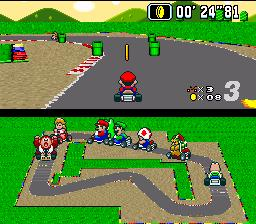
\includegraphics[scale=0.5]{imagenes/super_mario_kart.jpg}
          \end{center}
          Super Mario Kart - SNES (1992)
        \end{figure}
        
    \end{columns}
    
\end{frame}
